\documentclass[11pt]{article}

\usepackage[margin=1in]{geometry}
\usepackage{amsmath,booktabs,array}
\usepackage{graphicx}
\usepackage[hidelinks]{hyperref}
\usepackage{xcolor}
\usepackage{enumitem}
\usepackage{amsfonts}

\setlist[itemize]{leftmargin=1.5em,itemsep=0.25em,topsep=0.35em}
\setlist[enumerate]{leftmargin=1.8em,itemsep=0.25em,topsep=0.35em}
\newcommand{\code}[1]{\texttt{#1}}
\newcommand{\status}[1]{\textcolor{blue!65!black}{\textbf{#1}}}

\title{Racer-LLM Experiment Progress Log}
\author{}
\date{Last updated: August 25, 2026}

\begin{document}
\maketitle

\section{Project direction}

The main goal is to study the behavior and limitations of LLM-based policies in
a real-time multi-agent racing task. The baseline work is meant to provide
stable and understandable comparisons,instead of an exact
reproduction of every low-level detail in earlier racing systems of $\alpha$-racer or IBR from Wang et. al.. Should not diverge and get stuck in off-topic details, like tuning for better LLM agent performance.

The current comparison plans will eventually include:
\begin{itemize}
  \item locally trained and released $\alpha$-RACER policy;
  \item iterated best-response (IBR) policy;
  \item pure rule-based policy;
  \item LLM policy;
  \item LLM policy with explicit prompt rules.
\end{itemize}

The parameterized policies share the same local MPC and simulator wherever
possible. IBR is a separate online trajectory-optimization baseline and should
be described as such.

\section{August 10--12, 2026: local $\alpha$-RACER training}

\status{Status: implemented, trained, and provisionally validated.}

\subsection{$\alpha$-RACER in brief}

$\alpha$-RACER represents each car's high-level policy using five parameters
\[
  \theta_i=(q_i,\zeta_i,s_{1,i},s_{2,i},s_{3,i}).
\]
The parameters control how the MPC follows and modifies a precomputed
single-agent raceline, including tracking aggressiveness, speed along the
raceline, overtaking, and blocking behavior.

For a joint policy for three car $\theta=(\theta_0,\theta_1,\theta_2) \in \Theta^3$, car $i$ has a
long-term value
\[
  V_i(x,\theta)=\mathbb E\left[\sum_t\gamma^t r^i_t\right].
\]
In the paper they use artificial neuron network $\Phi$ to learn from generated racing records data and to approximate the changes of race state value respect to single agent variation:
\[
\begin{split}
  &\Phi(x,\theta'_i,\theta_{-i})-\Phi(x,\theta_i,\theta_{-i})\\
  &\qquad\approx
  V_i(x,\theta'_i,\theta_{-i})-V_i(x,\theta_i,\theta_{-i}).
\end{split}
\]
The function learned offline is later used in online policy searches for joint
parameters that give a high potential value and executes its own five-parameter
block.


\subsection{Local implementation}

The current implemented pipeline contains three
clearly separated stages.

\paragraph{1. Rollout collection.}
For each group, a baseline joint parameter set is sampled within the configured bounds of $(q,\zeta,s_1,s_2,s_3)$. Four races are simulated, resample the five control parameters of single agent:
\begin{enumerate}
  \item the baseline parameters for all three cars: $(\theta_0,\theta_1,\theta_2)$;
  \item a unilateral parameter change for car 0: $(\theta_0',\theta_1,\theta_2)$;
  \item a unilateral parameter change for car 1: $(\theta_0,\theta_1',\theta_2)$;
  \item a unilateral parameter change for car 2: $(\theta_0,\theta_1,\theta_2')$.
\end{enumerate}
Only one car's parameters change in each deviation race. This gives paired data
for learning the effect of unilateral policy changes.

At each control update, the code stores a 39-dimensional feature vector (relative progress, vehicle states, track curvature, and all 15 policy
parameters). The local single-step reward is currently the closing the gap or extending the lead against the fastest rivals, plus the safety term of off-road or collision penalty:
\[
  r^i_t=w_p\Delta s^i_t
  -w_o\mathbf{1}_{\mathrm{offroad},i}
  -w_c\mathbf{1}_{\mathrm{collision}}.
\]

The final feature data would be at the shape of ($N_{group}$, 4, time\_steps, 39). 4 represents 4 pairs of data per group and 39 represents the feature dimension as well as the size of the input for value function and potential function.

\paragraph{2. Value-function training.}
After a rollout finishes, discounted returns are computed backwards:
\[
  G^i_t=\sum_{k=t}^{T-1}\gamma^{k-t}r^i_k.
\]
And the value function $\widehat{V}_i(x,\theta)$ is trained using this Monte-Carlo learning to maximize the discounted accumulative returns $G_t$. The loss function:
\[
\mathcal{L}_{V_i}=\mathbf{MSE}(\widehat{V}_i(z_i),G^i_t)
\]

\paragraph{3. Potential-function training.}
The three trained value networks produce targets for unilateral value changes.
The potential network is trained so that
\[
  \widehat\Phi(x,\theta')-\widehat\Phi(x,\theta)
  \approx
  \widehat V_i(x,\theta')-\widehat V_i(x,\theta).
\]
Both sides are evaluated at the same baseline state. This avoids mixing a policy
change with the different state trajectory that the policy later causes.
The loss function:
\[
\mathcal{L}_{\Phi}=\mathbf{MSE}(\Delta \widehat V_i(x)-\Delta \widehat \Phi_i(x))
=
\frac{1}{\mathcal D_\Phi}\sum_{(x,\theta,\theta')}(\widehat V_i(x,\theta')-\widehat V_i(x,\theta),
\widehat\Phi(x,\theta')-\widehat\Phi(x,\theta))^2,
\]
Existing generated rollout data and trained checkpoints are reused automatically. If there is new rollout data the code would automatically re-train the later stage.

\subsection{Connection to the released code}

\begin{center}
\small
\begin{tabular}{p{0.20\linewidth}p{0.35\linewidth}p{0.35\linewidth}}
\toprule
Task & Released repository & Local project \\
\midrule
Collect races &
\code{collect\_data.bash}, \code{multi\_car\_blocking.py},
\code{merge\_data.py} &
\code{collect\_rollout\_data()} \\
Fit three values &
\code{train\_q\_model\_multi.py},
\code{train\_q\_model\_multi\_rel.py} &
\code{train\_value\_functions()} \\
Fit potential &
\code{train\_p\_model\_multi\_dist.py} &
\code{train\_potential\_function()} \\
Network definition &
\code{model\_arch.py::SimpleModel} &
\code{policy/alpha\_model.py::SimpleNeuralNetwork} \\
Online policy &
Released numerical simulator &
\code{policy/alpha\_racer.py::AlphaRacerPolicy} \\
\bottomrule
\end{tabular}
\end{center}

The local implementation keeps the original overall idea but exclude the ROS simulation dependency and change the chaining order of data pairs to more independent deviation groups of 4 shown previously.

\subsection{Training run recorded}

\begin{itemize}
  \item Track: Berlin.
  \item Vehicle model: local kinematic model.
  \item MPC horizon: 10.
  \item Data: 100 groups $\times$ 4 rollouts $\times$ 120 control samples.
  \item Rollout duration: 12 s.
  \item Discount: $\gamma=0.98$.
  \item Seed: 7.
  \item Value validation MSE: 21.43, 20.95, and 22.63.
  \item Best potential difference MSE: 0.0761.
\end{itemize}

\subsection{Initial three-position checkpoint comparison}

We make evaluation of locally trained weight using the standard three-position sweep on the Berlin track.
Each race(50s) contained three same $\alpha$-RACER cars.

\begin{center}
\small
\begin{tabular}{lcc}
\toprule
Checkpoint & Mean progress gain per car & Mean speed \\
\midrule
Released potential weights & 180.80 m & 3.56 m/s \\
Reimplementation trained & 198.64 m & 3.90 m/s \\
\bottomrule
\end{tabular} 
\end{center}

In shows that the locally trained checkpoint increased the mean
progress gain by 17.85 m and the mean speed by approximately 0.35 m/s. Neither configuration produced a recorded collision. The released checkpoint had no recorded off-road time, while the local checkpoint accumulated 0.08 seconds of off-road time across the nine vehicle trajectories.

These results show that the locally trained checkpoint runs successfully and
achieves higher progress under the local vehicle dynamics. It is therefore
suitable for use as the current $\alpha$-RACER baseline. 

\section{August 10--17, 2026: ordinary local IBR}

\status{Status: implemented and tested with SE disabled.}

The other thing we worked on was replacing the problematic IBR inherited from
the released $\alpha$-RACER code. The new version is based on the main idea in Wang et al.: iteratively update the planned trajectory against the opponent agent.

The current implementation does not copy Wang's low-level
solver but uses the state and controls already used in this project:
\[
  x_i=[s_i,e_i,\Delta\psi_i,v_i]^\top,
  \qquad
  u_i=[\text{throttle}_i,\text{steer}_i]^\top.
\]

Wang's ordinary IBR alternates best responses: one car optimizes its trajectory
while the other planned trajectories are fixed, and the updated plans are used
in the next round. Its racing objective mainly rewards progress, while vehicle
dynamics, track containment, and collision avoidance define the feasible
trajectories. We keep this general structure but use the local kinematic model
rather than Wang's trajectory parameterization and low-level solver.

Given N as the prediction horizon, the objective used for the current local baseline is
\[
\begin{aligned}
J_i={}&-w_p(s_{i,N}-s_{i,0})
  +w_e\sum_{k=0}^{N-1}e_{i,k}^4\\
&+w_{\Delta u}\sum_{k=0}^{N-1}\|u_{i,k}-u_{i,k-1}\|_2^2\\
&+\rho_t\|\epsilon_t\|_2^2
  +\rho_c\|\epsilon_c\|_2^2.
\end{aligned}
\]
The weights are $w_p=10$, $w_e=10$, and $w_{\Delta u}=0.10$. The
fourth-power lateral term follows the form used by the released
$\alpha$-RACER IBR. It is small near the centre of the track but grows rapidly
near the boundary. The control-rate term is a standard local regularizer that
reduces abrupt command changes. We removed the earlier
$\|u-u_{\mathrm{neutral}}\|^2$ term because its neutral command was a local
design choice and was not needed by the tests.

It also shares the constraints with the local kinematic model and vehicle
parameters, uses normalized throttle and steering bounds, maximum speed,
steering-rate limit, and the same friction-based steering/speed limit used by
the local MPC. Track and collision constraints have explicit nonnegative slack
variables with large penalties. These are local feasibility devices rather
than part of Wang's original hard-constrained formulation, and their activation
is recorded.

\subsection{Objective and slack audit}

We selected the objective using six scenarios: the three Berlin starting
positions, a Berlin closing-speed case, and one case each on the Modena and
rounded-rectangle tracks. The table reports mean per-car progress gain and
aggregate event time over the six simulations.

\begin{table}[ht]
  \centering
  \small
  \begin{tabular}{lrrrr}
    \toprule
    IBR variant & Progress (m) & Off-road (s) & Collision (s) & Solver failure (s) \\
    \midrule
    Progress only & 82.24 & 11.42 & 1.58 & 0.10 \\
    $+\|\Delta u\|^2$ & 82.16 & 13.64 & 2.62 & 0.00 \\
    $+0.4e^2+\|\Delta u\|^2$ & 82.96 & 0.28 & 1.52 & 0.00 \\
    $+10e^4+\|\Delta u\|^2$ & 82.84 & 0.00 & 1.36 & 0.00 \\
    $e^2$, hard track constraint & 65.55 & 54.94 & 2.66 & 72.80 \\
    $e^2$, hard collision constraint & 83.32 & 0.00 & 1.10 & 1.20 \\
    $e^2$, both constraints hard & 57.09 & 80.80 & 24.58 & 110.80 \\
    \bottomrule
  \end{tabular}
  \caption{Local IBR objective and feasibility audit over six scenarios.}
\end{table}

The progress-only planner exploited the track boundary. A control-rate penalty
made the commands smoother but did not solve this problem. Both $e^2$ and
$e^4$ removed almost all off-road motion without materially reducing progress;
we retained $10e^4$ because it has a direct precedent in the released
$\alpha$-RACER IBR and gave zero recorded off-road time in this test.

Removing track slack caused repeated infeasibility and recovery loops. Removing
collision slack caused shorter, localized solver failures in close packs.
Therefore both slacks remain enabled, with their values logged so that they
cannot silently substitute for safe behavior.

\section{August 13--15, 2026: initial policy-abstraction comparison}

We compared four ways of producing the five parameters used by the shared
low-level MPC. The raw LLM and rule-prompt LLM select from four manually defined
$\alpha$-RACER modes; the rule-only policy executes the same explicit rules
without an LLM; and the direct-parameter LLM outputs
$(q,\zeta,s_1,s_2,s_3)$ within their configured bounds. Each policy was tested
from all three starting positions against two local $\alpha$-RACER cars and
then against two IBR cars.

The IBR comparisons were run before the final objective audit and are retained
as preliminary single-run observations. They will be repeated over multiple
trials for the final evaluation.

\begin{table}[ht]
  \centering
  \small
  \begin{tabular}{lcccc}
    \toprule
    & \multicolumn{2}{c}{vs. local $\alpha$-RACER}
    & \multicolumn{2}{c}{vs. IBR} \\
    \cmidrule(lr){2-3}\cmidrule(lr){4-5}
    Policy & Wins & Progress (m) & Wins & Progress (m) \\
    \midrule
    Raw LLM          & 2/3 & 193.2 & 0/3 & 193.1 \\
    Rule-prompt LLM  & 0/3 & 111.3 & 0/3 & 161.6 \\
    Rule-only policy & 0/3 & 134.8 & 0/3 & 171.8 \\
    Direct-parameter LLM & 0/3 & 177.0 & 0/3 & 177.4 \\
    Local $\alpha$-RACER self-play & 1/3 & 193.0 & -- & -- \\
    \bottomrule
  \end{tabular}
  \caption{Mean ego progress over the three starting positions.}
\end{table}

The raw mode-selecting LLM was close to local $\alpha$-RACER in progress. The
explicit rules made both the rule-prompt LLM and deterministic policy too
conservative: they selected \emph{stable} frequently even though it is not a
dedicated recovery controller. The direct-parameter LLM performed between the
raw LLM and rule-based variants, but did not use the available parameter space
adaptively.

\begin{figure}[ht]
  \centering
  \includegraphics[width=\textwidth]{figures/direct_param_distribution.pdf}
  \caption{Parameter choices aggregated over all six races (300 LLM
  decisions). Bars show discrete selection frequencies after rounding only
  numerical precision.}
  \label{fig:direct-param-distribution}
\end{figure}

Figure~\ref{fig:direct-param-distribution} makes this concentration visible:
$q=2.8$ was selected in 256 of 300 decisions and $s_1=0.4$ in 231. This suggests
that, for this model and prompt, mapping a numerical scene directly to five
coupled MPC parameters is harder than selecting a semantic mode. It does not
show that the manually chosen mode presets are optimal; these can later be
calibrated on a separate scenario set without changing the mode selector or
final test set.

None of the LLM variants met the one-second decision interval. Raw prompts took
approximately 3--4 s, rule prompts 4--5 s, and direct-parameter prompts about
7 s per call. The raw LLM was the strongest preliminary variant, but it also
showed occasional contact or off-road recovery.

These were preliminary results with the earlier shared MPC. The updated
controller results below show that the low-level formulation can change the
relative performance of the high-level policies.

\section{August 22--25, 2026: shared MPC stall investigation}

After correcting the local steering calibration and regenerating the raceline,
several parameterized policies repeatedly stopped near the same Berlin hairpin,
at approximately $64$--$65$ m progress. The NLP solver normally reported a
successful solution, so this was not primarily a solver-crash problem.

The useful diagnosis was that the four-state kinematic model has yaw rate
proportional to speed. At very low speed the car must accelerate before steering
can change its trajectory. In the difficult hairpin state, this initially
increases tracking or constraint cost, while a nearly neutral first command
keeps the immediate cost small. Receding-horizon replanning can then repeatedly
postpone the acceleration shown later in the predicted plan.

Longer horizons, alternative initial guesses, terminal turning-room penalties,
and a history-dependent stall penalty were tested as diagnostics. They changed
the predicted plans but did not reliably remove the stopped solution. Hardening
the softened track constraint caused infeasibility in difficult states, while
loosening it too much allowed the optimizer to leave the track. These negative
tests are not proposed as new methods; they helped isolate the problem before
changing the main controller.

\subsection{Check against the released numerical project}

We also ran the unmodified released $\alpha$-RACER numerical race callback in a
headless wrapper. ROS publishers and visualization messages were replaced by
empty adapters, but the released dynamics, MPC, IBR, checkpoints, initial
states, $0.1$ s update, and 500-step race loop were retained. ROS is therefore
not required for the numerical algorithms themselves.

The released simulator explicitly intervenes after $|e|>0.55$ m by reducing
velocity, rotating the vehicle toward the reference, and adding inward steering.
The following single-race checks show that this recovery is used materially.

\begin{table}[ht]
  \centering
  \small
  \begin{tabular}{lrrr}
    \toprule
    Released setup & Final progress (m) & Maximum $|e|$ (m) & Time $|e|>0.55$ (s) \\
    \midrule
    $\alpha$-RACER vs. MPC vs. MPC
      & $110.4/84.1/117.1$ & $0.867/0.812/0.585$ & $13.3/8.3/1.2$ \\
    $\alpha$-RACER vs. IBR vs. IBR
      & $108.8/120.3/73.5$ & $0.873/0.940/1.315$ & $15.7/10.1/22.3$ \\
    \bottomrule
  \end{tabular}
  \caption{Headless execution of two released 50 s numerical races. Values are
  shown in car order.}
\end{table}

This does not make the local stall desirable, but it changes the interpretation:
the released implementation also does not rely on its MPC or IBR alone to remain
on track. Its simulator-level recovery is an important part of completing a
race. For the local primary comparison, the low-speed recovery supervisor remains
disabled so that policy failures are not silently corrected.

\section{August 25, 2026: reference-speed tracking update}

The shared MPC originally tracked moving raceline positions but had no explicit
penalty on the supplied raceline speed. We added the conventional term
\[
  J_v=w_v\sum_{k=0}^{N}(v_k-v_k^{\mathrm{ref}})^2.
\]
It is shared by the LLM, rule-based, $\alpha$-RACER, and Parameter-IBR policies.
The final small screen retained the original horizon $N=10$ and track-slack
weight $10^4$, and selected $w_v=10$. In the difficult Position-3 rule-policy
screen, weights $1$, $3$, and $10$ all passed the hairpin; their progress was
$89.1$, $95.2$, and $98.0$ m respectively, with no recovery activation. The
$w_v=10$ run also stayed within the nominal $0.44$ m boundary.

Reducing the track-slack weight was not necessary. With $N=20$, $w_v=10$, and
slack weight $10^3$, the car progressed but reached $|e|=0.649$ m and activated
recovery. Restoring the slack weight to $10^4$ gave $98.8$ m progress without
crossing the nominal boundary. This supports keeping the original safety weight
rather than solving the stall by making departures cheap.

\subsection{Three-position regression}

The table summarizes the updated three-position tests against two locally
trained $\alpha$-RACER cars. ``Stall'' denotes an ego car finishing near zero
speed at the hairpin. Each position was run once, so the table is a regression
check rather than a final statistical evaluation.

\begin{table}[ht]
  \centering
  \small
  \begin{tabular}{lrrrr}
    \toprule
    Ego policy & Wins & Mean progress (m) & Ego stalls & Recovery time (s) \\
    \midrule
    Local $\alpha$-RACER self-play & 1/3 & 99.6 & 0 & 0.00 \\
    Pure rule-based                 & 1/3 & 103.5 & 0 & 0.00 \\
    Raw LLM                         & 0/3 & 86.8 & 1 & 0.22 \\
    Rule-prompt LLM                 & 1/3 & 103.9 & 0 & 0.00 \\
    Parameter-IBR                   & 1/3 & 89.1 & 1 & 0.02 \\
    \bottomrule
  \end{tabular}
  \caption{Updated shared-MPC regression with $N=10$, $w_v=10$, and track-slack
  weight $10^4$.}
\end{table}

\begin{figure}[ht]
  \centering
  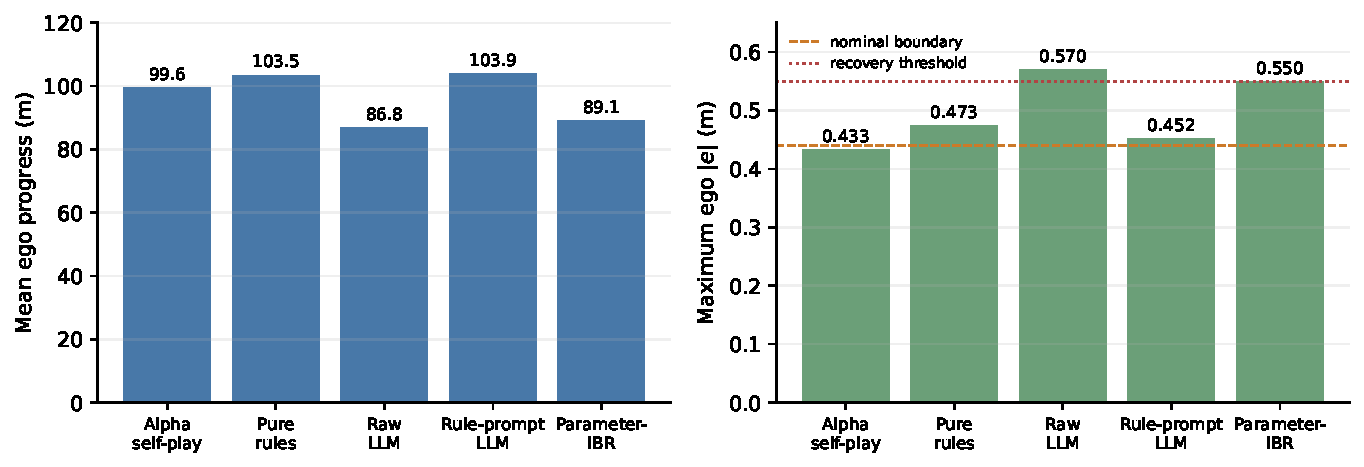
\includegraphics[width=0.96\textwidth]{figures/august25_shared_mpc_comparison.pdf}
  \caption{Mean ego progress and maximum ego lateral error across the three
  starting positions. The dashed and dotted lines mark the local nominal
  boundary and released-simulator recovery threshold.}
  \label{fig:august25-shared-mpc}
\end{figure}

The updated controller removed the earlier widespread stall in $\alpha$-RACER
self-play and in the rule-policy ego runs, without requiring the experimental
terminal or stall-debt penalties. It did not make every high-level reference
recoverable: raw LLM and Parameter-IBR each still produced one hairpin stall.
The remaining failures are therefore treated as outcomes of particular
high-level/reference interactions rather than hidden by another recovery rule.

The policy ordering also changed. The raw LLM selected \emph{push} almost all the
time and stalled from Position 3. The rule-prompt LLM selected mostly
\emph{stable}, completed all three races, and performed similarly to the pure
rule policy. This means the earlier conclusion that explicit rules were simply
too conservative was dependent on the earlier low-level controller. A larger,
held-out comparison is required before making a final prompt claim.

LLM timing remains unresolved. All 75 calls in each prompt condition missed the
one-second decision interval. Raw calls averaged approximately $2.8$ s, while
the longer rule prompt averaged approximately $4.4$ s. The simulator currently
waits for each response, so these tests measure decision quality but not the
physical effect of delayed execution.

The next analysis will separate scene understanding from preset quality. Saved
observations can be labelled automatically for road geometry, boundary risk,
front/rear traffic, gap, and closing speed; mode choices and short explanations
can then be checked offline before changing either the prompt or the four manual
mode presets.

\section{How IBR will be used in the comparison}

IBR does not solve the same control problem as the high-level policies.
$\alpha$-RACER and the LLM policies select five parameters and share a
low-level MPC that follows moving raceline-based position and speed references.
The initial experiments above used zero velocity-error weight; after the stall
investigation the shared controller uses the explicit speed-tracking term with
$w_v=10$. This remains a soft objective rather than a hard speed limit.

The local IBR instead selects throttle and steering directly and rewards
progress. Wang's IBR likewise optimizes racing trajectories rather than
following the local $\alpha$-RACER speed profile. With only the simulator's
global $5\,\mathrm{m/s}$ bound, local IBR can consequently drive near that
limit for most of a lap. This gives it a different speed opportunity as well as
a different action space.

\begin{table}[ht]
  \centering
  \small
  \begin{tabular}{lccc}
    \toprule
    Candidate against local $\alpha$-RACER & Wins & Progress (m) & Speed (m/s) \\
    \midrule
    IBR, global speed limit    & 3/3 & 237.3 & 4.74 \\
    IBR, raceline-speed constrained & 0/3 & 183.0 & 3.61 \\
    Local $\alpha$-RACER self-play & 1/3 & 193.0 & 3.91 \\
    \bottomrule
  \end{tabular}
  \caption{Preliminary single-run results using the pre-audit IBR objective.}
\end{table}

The existing ``raceline-speed constrained'' implementation applies a bound that
tightens toward $1.04$ times the raceline speed while allowing the minimum
speed reachable under full braking. It substantially reduced IBR performance,
but it is not exactly equivalent to the indirect way in which the shared MPC
uses the profile. The table is therefore evidence that speed access explains a
large part of the IBR advantage, not yet a definitive fair comparison.

The unrestricted IBR will be kept as a strong full-trajectory optimization
reference. Its wins do not by themselves show better interaction reasoning
than the LLM. The main like-for-like comparison remains the LLM, rule-prompt
LLM, rule-only policy, and $\alpha$-RACER, which share the five-parameter action
space and low-level MPC.

Before finalizing the speed-controlled IBR ablation, we should decide whether
it should use (i) the present physically relaxed speed bound, (ii) a soft
penalty only for exceeding the raceline profile, or (iii) an explicit velocity
tracking term. This choice should be discussed because Wang does not require
the local raceline profile, while imposing it too strongly changes IBR from a
free trajectory optimizer into a raceline follower. Whichever definition is
chosen will be fixed before the final multi-seed evaluation; the earlier
single-run IBR comparisons will then be rerun with the audited objective.

\end{document}
